%!TEX root = thesis.tex
In the previous chapters we have investigated our initial interpretation of AHIs though inspirational user studies and prototyping.
Our initial thoughts on AHIs were based on existing research directions and inspiration from the domestic domain which led us the idea of AHIs as a novel interaction approach that, in our optics, touches upon some little unexplored areas of HCI.  
As we have now gone through three very different approaches to creating AHIs it is now time to zoom out from the individual details of the approaches and revisit our concept of AHIs based on our experiences, both the successful and the less successful.
\todo{mere indledning}


\section{Understanding interaction with AHIs}
\begin{quotation}
\emph{When Koffka asserted that ``each thing says what it is'' he failed to mention that it may lie. More exactly, a thing may not look like what it is \citep{gibson1979ecological}.}
\end{quotation}
The above quote from \citeauthor{gibson1979ecological} is especially interesting in relation to AHIs as it points to a challenge that we have not really touched upon in this thesis.
As AHIs have an inherently dynamic nature how do we ``pick up'' the interaction possibilities of the interface? 
In the following we will take a look at our experiences with AHIs in the light of affordance theories to assert whether affordances can help communicate intent in such dynamic interfaces as AHIs and point to possible areas of improvement.

\subsubsection{Affordances}
The notion of affordances describes the relationship between the acting organism and the acted-upon environment.
The term comes from the above cited perceptual psychologist J.J. Gibson.
Affordances are properties of the environment that, for good or ill, tells us about the possible actions that are available to us.
Affordances therefore describe the potentials for actions in the environment as we perceive that environment.  

\subsubsection{Perception and Affordances}
Perception is a key concept in relation to affordances as in order to ``know'' an affordance is there, you have to perceive it with your senses. Where \citet{gibson1979ecological} focuses mostly on visual perception, \citet{gaver1991technology} wants to broaden it to include all the senses, such as tactile and auditory feedback.
For example, sound can be used to indicate affordances that cannot be seen, where the sound of a turning lock indicates that the affordance of the door has changed.

\citet{gaver1991technology} notes that \emph{``Affordances per se are independent of perception''}.
This separation of affordances and the information available about them to us, gives rise to complications, as affordances will still exists even if you do not perceive them or if you perceive them wrong.
Additionally you might perceive an affordance that does not exist.

This leads back the the opening quotation from Gibson as there, in the case of AHIs, is a possibility that an object does not have perceivable affordances that match the actual affordances.
If we look at our first AHI construction approach that we suggested in chapter~\ref{ch:adhoc}, we proposed an approach where objects changes their shape.
Dynamic shapes would allow for dynamic, or changing, affordances where the perceived action possibilities of an object would change based on the change in shape.
So one form instance of a dynamic objects does not necessarily allow the for the perceptibly of all the possible affordances of that object, leading to, in Gaver's term, hidden affordances. 
The same is true for our embedded invisible interfaces where the perceived affordances will most likely be tied to the object in which the interface is embedded and not the interface itself.

So Gibson's focus on what can be \emph{seen} does not fit dynamic objects.
Gaver suggests a more exploratory approach for interfaces with complex affordances, which is where AHIs fit, where the affordances are learned through use and interaction.
\hl{The notion of learning through use is especially relevant for our Textile Touch as we envision this as an interface that should be an unconscious extension of the }

The exploratory approach is taken up by \citet{djajadiningrat2004tangible} who suggests a focus on both appearance and action as carriers of meaning.

\subsubsection{Appearance and Action}
Another way to approach the question about how objects appeal to our senses and motor skills is presented by \citet{djajadiningrat2004tangible}.
As we have seen above traditional focus of affordance concerns appearance and action, where affordances invite an arbitrary action. 
In this sense it is the appearance, both visual and physical, of an object that carries the meaning.

\citeauthor{djajadiningrat2004tangible} argues for an approach where the focus in on \emph{both} appearance and action as carriers of meaning, inextricably linking usability and aesthetics.
In this way action and appearance both expresses something about the purpose of the interface and they identifies two options for creating meaning through this expressiveness, a semantic and a direct.

In the \emph{semantic} approach meaning is derived from semantics and cognition.
So metaphors, for example, can trigger associations to other products or concepts with which the user is familiar.
This approach is somewhat in play in Textile Touch as the interaction should, ideally, draw on the common touch interaction patterns that are prevalent in today's smart phones and tablets.
In retrospect this should have had more focus in our test application for Textile Touch as some of our patterns were too disconnected from the action they performed creating a mismatch between the expected outcome and the actual outcome.
Further work on this could with advantage refer to \citep{wobbrock2009user,morris2010understanding} for an understanding of gestures and user generated gestures.

In the \emph{direct} approach meaning is created in the interaction with physical objects and therefore there is a strong emphasis on the perceptual and bodily skills of the user.
The idea is that meaning is created in interaction, much resembling Gaver's `learning through use'. 
This could be one way to understand shape changing AHIs as they their action possibilities shifts with changes in form, especially if the user is the manipulator of form.
One thing we noticed when experimenting with shape change, both in chapter~\ref{ch:workshops} and \ref{ch:jamming}, was that it was quite hard to agree on forms when the interface had many degrees of freedom.
So given a ``blob'' that could deform in any way, in our case a piece of plasticine, we saw difficulties in continuously recreating the same forms, which would be needed for a direct mapping between form and function.
This is problematic as it would make it hard to ``learn'' the interface if forms are hard to consistently match.
So in order to create meaning in interaction for such interfaces we see the need for constrains to the number of possible forms that can be made, in that way retaining the physical exploration but in a limited fashion.

As we have only experimented with this briefly, it is hard to base a conclusion on our work.
Interestingly \citet{lee2010users} has made a study on the physical deformation and the related action that the deformation maps to, and find that the agreement on the mapping \emph{increases} with higher degrees of freedom, which seems counter intuitive.
Whether this finding can be transferred to 3D objects, which are inherently more complex than paper, would be interesting to test in a more thorough setting than ours.
While we do not anticipate that it would be true for a free-form object, perhaps there exists a middle ground between a certain amount of form constraints and form freedom that proves to give a more effective mapping between form an function.
\blank
Our conductive paint exploration from chapter~\ref{ch:prototype3} is quite different from the other two approach in terms of affordances.
As it is up to the user to construct the interface there is no initial perceptual or tangible guidelines to direct interaction or construction. Though the interesting aspect of our example of painting the wires and switches on the walls, is that it creates a, in Norman's terms \citep{norman2002design}, \emph{natural mapping} between the interface control and the controlled object as there would be a direct visual link between the two.
If this would lead to natural interaction is only speculative but it does point to a possible quality of such interfaces. 

\subsubsection{Feedback and Feedforward}
Another way to support the interaction and understanding of the interface can be done through feedback and feedforward.
The Interaction Frogger framework \citep{stienstra2012design,wensveen2004interaction} gives us a tool to understand and spot where improvements can be made in relation to feedback and feedforward.

\todo{inherent, functional, augmented feeback and feedforward}

\subsubsection{A taxonomy for tangibles}
The last topic we will cover in this section is short look on Fishkin's taxonomy for tangible interfaces \citep{fishkin2004taxonomy}.
The taxonomy uses two axes, \emph{metaphor} and \emph{embodiment} to address how `tangible' an interface is.
\emph{Embodiment} describes the relationship between the input focus and the output focus, while \emph{metaphor} describes the level of metaphorical ties the interface has, that is the level of a real-world analogy the interface has.

So can we, based on our prototypes and concepts, say something general about AHIs in terms of this taxonomy?
In figure~\ref{fig:ch:adhoc2:fishkin} we have placed our various AHIs to give an overview and look for eventual tendencies. 

\begin{figure}[h]
  \centering
  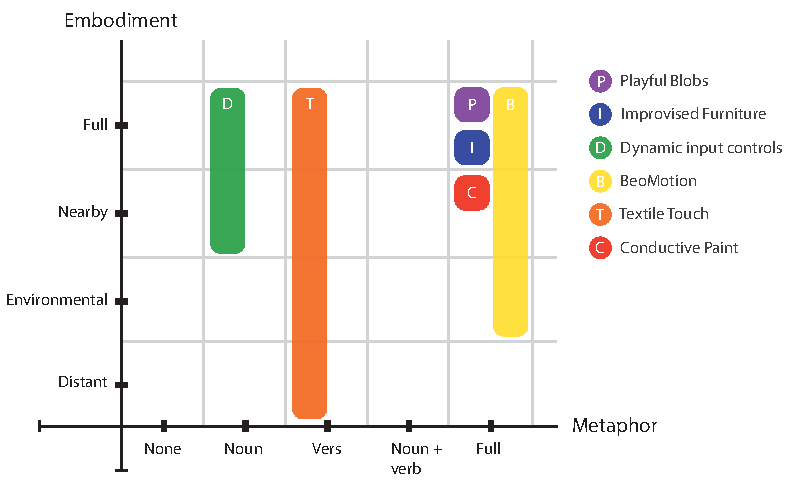
\includegraphics[width=.9\textwidth]{figures/adhoc2/fishkin.pdf}
  \caption{Placements of our prototypes and concepts in Fishkins taxonomi for tangible interfaces.}
  \label{fig:ch:adhoc2:fishkin}
\end{figure}

While it was more or less straight-forward to place the different prototypes and concepts on the scale of embodiment, it was a lot less given on the scale of metaphor.
As can be seen there is a tendency for a high degree of embodiment.
In Textile Touch we find that it depends quite a lot on the use situation as to how embodied the interface is.
While we envision situations and applications where the feedback and content is on the Textile Touch surface, where there would be a high degree of embodiment, other applications, such as controlling appliances in the near surrounding would have a lesser degree of embodiment.
The AHIs that involves shape-change generally shows a high degree of embodiment when change of shape is used for both input and output.

The placements on the metaphor axis are less certain.
One of the challenges here is that Fishkin focuses on real-world analogies.
So in our Playful Blobs for example we actually use digital-world analogies, such as \emph{copy/paste}, \emph{save} and \emph{open}, to describe real-world interaction.
So either we have \emph{no} metaphor, as there a no real-world analogy, or we bend the taxonomy a little and use \emph{verb} and accept the digital-world analogy for our tangible interface, or lastly we could see it as a \emph{full} metaphor as the virtual system \emph{is} the
physical system. 
We have placed it as a full metaphor as we argue that we have truly direct manipulation in the interface, merging the physical and digital system.

Generally we do see a high degree of tangibility in AHIs, at least based on our interpretation of the taxonomy, which does fit our goal of such interfaces as we seek to tie the physical and digital aspects of interfaces closer together, drawing on the qualities of both worlds.
The individual placements can of course be discussed as some of the examples could possibly have a different placement, but we do see a tendency in AHIs towards \emph{more tangibility} rather than less tangibility. 

\section{Knowledge construction}
\todo{eller research perspective eller \dots}

\begin{verbatim}
1. Projektet i lyset af Zimmermans 4 linser
* Process, invention, relevans, extensibility

2. perspektiver til ``Strong concepts''
* generativitet
* abstraktion

a look back: the interfaces have embedded function or meaning outside of interaction

Jamming: hvad har vi laert ifht AHIs
\end{verbatim}

\section{Perspectives}
\todo{maaske anden overskrift}

\citet{abowd2012next} notes that, while many of Weiser's predications about the future of computing has come true, some were not so accurate such as inch-scaled devices being readily disposable.
While this is true, our concept of AHIs does, in some aspects, challenge this as we propose that AHIs \emph{disappears} after use.
We see this disappearance both in the sense of the affordance or perception of the interface disappears, so here not a physical disposal in the sense that \citeauthor{abowd2012next} is referring to, but also in the sense of the physical removal of the interface.
This will most likely be most apparent in our third construction approach to AHIs as we here suggest that interfaces are build on the spot which will, at least in some cases, also lead to deconstruction of the interface after use and therefore be disposable in the sense \citeauthor{abowd2012next} is referring to.

As we saw with our exploration of paint as a construction mechanism the interface could be disposed simply with a wet cloth.
From a sustainability point of view disposable interfaces are of course not a \hl{positive} approach so such interfaces should instead focus on reuse, in our paint interface this could for example mean that the paint is collected in a container for later use instead of simply being washed away. 

\section{A possible fourth approach}
In our exploratory evaluation of Textile Touch we saw a pointer to a way of approaching AHIs that we had not considered in our initial outlay of the concept.

\todo{reference back to evaluation} 

Where we with the Textile Touch prototype have focused on it as an example of how interaction can be integrated into the existing environment in a ubiquitous fashion, it can also be used as an example of how to extend the capabilities of existing objects and augment its functions in an ad hoc manner.

At a glance this does sound somewhat like Augmented Reality (AR), but as \citet{azuma1997survey} describes it AR \emph{allows the user to see the real world, with virtual objects superimposed upon or composited with the real world.}
So the focus is on augmenting the environment virtually, while our focus is on augmenting the environment physically.

\todo{more on why this is so}

Inspired by this idea of augmenting existing objects in an ad hoc fashion we have taken a brief look around for other examples that might give weight to this approach.

REVEL \citep{bau2013revel}, as we have briefly mentioned earlier, is a system that via a digital overlay augments objects by changing the tactile perception of their physical surface.
So it is a physical augmentation that, in principle, can be done to arbitrary objects giving them a new function when part of the interaction, while retaining the existing properties of the object \todo{reformulate - focus on the aspect of the object being useful while augmented}

Another example is Pinoky \citep{sugiura2012pinoky} that is a wireless ring-like device that can augment ordinary plush toys to allow them to move limbs.
This is done by attaching the ring around a limb to actuate it and the Pinoky can now record movements done by the user and play them back, animating the plush toy.
